\lstset{
	basicstyle=\ttfamily,
	numbers=left,
	numberstyle=\color{gray},
	tabsize=2,
	language=C,
	morekeywords={exec,sql}
}
\begin{document}
\lecture{Implementierung von Datenbanksystemen}{IDB}
\title{Übungsblatt~8}
\subtitle{Programmzugriff, Transaktionen}
\maketitle

\beamertxt{\pagebreak}
\section*{Lernziele}

\begin{itemize}
  \item Erstellung und algebraische Optimierung von Ausführungsplänen mit Sichten
  \item Optimierung in der Praxis
\end{itemize}

\section*{Literatur}

\HaerderNintyNine{11, 12}

\ElmasriSeventh{18, 19}

\GarciaMolinaSecond{8, 15, 16}

\NeumannFifteen


\beamertxt{\pagebreak}
\section{Fragen zur Vorlesung -- Programmschnittstellen}

\begin{enumerate}[a)]
	\item Welche Vor- und Nachteile bringt die Verwendung eines Vorübersetzers zur Einbettung von SQL-Abfragen in Programmcode mit sich?

	\begin{solution}
	Vorteile:
	\begin{itemize}
		\item Kompakt zu programmieren.
		\item SQL-Anweisung wird zur Compile-Zeit geprüft, analysiert, optimiert, daher schnell und viele Fehler können schon zur Übersetzungszeit gefunden werden.
	\end{itemize}
	Nachteile:
	\begin{itemize}
		\item Spezieller Vorübersetzer für die Kombination aus Programmiersprache und DBMS notwendig.
		\item Häufig kein Standard-SQL, sondern mit syntaktischen Änderungen.
	\end{itemize}
	\end{solution}

	\begin{note}
	\begin{center}
	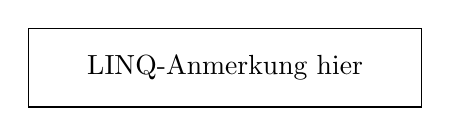
\begin{tikzpicture}
		\draw (0, 0) rectangle+(5, 1);
		\node at (2.5, 0.5) {LINQ-Anmerkung hier};
	\end{tikzpicture}
	\end{center}
	\end{note}

	\item Warum benötigt man bei Datenbankzugriffen aus Programmcode heraus in der Regel Cursor?

	\begin{solution}
	Da Programme im Allgemeinen mit einzelnen Werten arbeiten, Datenbanken aber mit einer Mengensemantik, ist es in der Regel so, dass Anfragen eine Ergebnismenge zurückliefern und nicht einzelne Werte.
	Um diese verarbeiten zu können, benötigt man eine Art Schleife über der Ergebnismenge, dies ist der Cursor. Mit diesem wird die Ergebnismenge in der Regel zeilenweise abgearbeitet; wobei nun jede Zeile in einzelne Werte zerlegt werden kann (Stichwort for-each-Schleife).
	\end{solution}

\end{enumerate}

\beamertxt{\pagebreak}
\section{Programmschnittstelle}

Gegeben sei folgende SQL-Abfrage:

\texttt{SELECT nachname, vorname FROM Kunden WHERE kundennr = 23;}

An der internen Satzschnittstelle stehen folgende Objekte zur Verfügung:
\begin{itemize}
	\item eine Datei \emph{Kunden}, die die Kundendatensätze in Form von Tupeln der Relation enthält;
	\item eine Datei \emph{Kundennummer-Index}, die eine Kundennummer auf eine Satzadresse abbildet.
\end{itemize}
Jede Kundennummer ist eindeutig.

\begin{enumerate}[a)]
	\item Schreiben Sie ein Programm, dass die o.\,g.\ SQL-Anfrage mit den Aufrufen der internen Satzschnittstelle realisiert. Verwenden Sie eine Sprache Ihrer Wahl oder auch Pseudocode.

	\begin{solution}
	%TODO Fehlerbehandlung
	\nt{TODO: Fehlerbehandlung!}
	\texttt{// Wir nehmen an, dass der Eintrag existiert\\
		// Es wird auf eine Fehlerbehandlung verzichtet\\
		//[Skript S. 5-34] \\
		KeyedRecordFile index = new KeyedRecordFile("Kundennummer-Index", "r"); \\
		TID tid = index.read-key(23); \\
		//[Skript S. 3-28] \\
		DirectRecordFile saetze = new DirectRecordFile("Kunden", "r"); \\
		Record ergebnis = saetze.read(tid); \\
		ergebnis = ergebnis.proj("nachname", "vorname"); \\
		print(record\_to\_string(ergebnis));}

	Oder alternativ etwas C-näher:

	\texttt{FILE *index = keyed\_record\_file\_open("Kundennummer-Index", "r"); \\
		TID tid; \\
		keyed\_record\_file\_read-key(index, 23, \&tid, sizeof(tid)); \\
		//[Skript S. 3-28] \\
		FILE *saetze = direct\_record\_file\_open ("Kunden", "r"); \\
		Record ergebnis; \\
		direct\_record\_file\_read(saetze, tid, \&ergebnis, sizeof(ergebnis)); \\
		record\_project(\&ergebnis, sizeof(ergebnis), "nachname", "vorname"); \\
		printf(record\_to\_string(ergebnis));}
	\end{solution}

	\item Wie würde das Programm aussehen, wenn kein Index zur Verfügung stünde?

	\begin{solution}
		\texttt{
			\begin{tabbing}
			\hspace*{1cm} \= \hspace*{1cm} \= \kill
			//[Skript S. 3-28] \\
			DirectRecordFile saetze = new DirectRecordFile("Kunden", "r"); \\
			Record ergebnis; \\
			while (saetze.hasNext()) \{ \\
			\> ergebnis = saetze.next(); \\
			\> if (ergebnis.get(kundennr) == 23) \{ \\
			\> \> ergebnis = ergebnis.proj("nachname", "vorname"); \\
			\> \> print(record\_to\_string(ergebnis)); \\
			\> \> break; //Abbruch, jede Kundennummer existiert 1x \\
			\> \} \\
			\}
			\end{tabbing}
		}
	\end{solution}

	\item Was muss (in groben Zügen) anhand der SQL-Anfrage geprüft und ermittelt werden, damit ein lauffähiges Programm entsteht?

	\begin{solution}
	\begin{itemize}
		\item Syntaxprüfung
		\item Gibt es die Relationen und Attribute überhaupt?
		\item Wie heißt die Datei zur Relation?
		\item Was für eine Datei ist das –- direkt oder Schlüssel-basiert?
		\item Gibt es einen Index für "`kundennr"'?
		\item Wie heißt dessen Datei?
		\item Wie lang sind die Sätze der Datei "`Kunden"'?
	\end{itemize}
  Die Diskussion, was davon zur Übersetzungs- und was zur Laufzeit durchgeführt wird, führen wir detaillierter in Übung 10 zur Anfrageverarbeitung.
	\end{solution}

	\item Welche Methoden sollte ein Call-Level Interface bieten, das die Ausführung von SQL-Anfragen ermöglicht?

	\begin{solution}
	Das ist das Prinzip jeder DB-Schnittstelle, z.\,B.\ in PHP, Java/JDBC, C\#ODP.NET, usw. Die Verbindung sei schon gegeben (z.\,B.\ via \texttt{connect(username, password, database}).

	Dann benötigen wir:
	\begin{enumerate}[i)]
		\item eine Methode, um eine Abfrage auszuführen (Diese sollte einen Status über die Ausführung der Query bzw. ein Handle zum Abrufen des Ergebnisses liefern.);
		\item eine Methode um zu prüfen, ob es (weitere) Ergebnisse gibt;
		\item eine Methode, um überhaupt an die Ergebnisse heranzukommen.
	\end{enumerate}

	Ein Beispiel (JDBC):
	\begin{enumerate}[i)]
		\item \texttt{ResultSet Statement.executeQuery(String query);}\\
		Wirft im Fehlerfall eine Exception.
		\item \texttt{Boolean ResultSet.next();}\\
		Bewegt den Zeiger auf das nächste Ergebnis, \texttt{true} bei Erfolg, \texttt{false} sonst.
		\item \texttt{Record ResultSet.[getString, getInt, \ldots](int columnIndex);}\\
		Liefert den zugehörigen Wert im aktuellen Ergebnis.
	\end{enumerate}

	\end{solution}
\beamertxt{\pagebreak}

	\item Bei einem Call-Level Interface kann die ganze Bearbeitung der Anfrage erst zur Laufzeit erfolgen. Dabei wird auch ein Programm erzeugt, für das die oben eingeführten Pseudocode-Programme als Beispiel genommen werden können.

	Eine clevere Idee ist nun, die Programme aufzubewahren und bei zukünftigen SQL-Anfragen zu prüfen, ob sie nicht auch dafür verwendet werden können. Dies erlaubt es, den Aufwand der Neuerzeugung einzusparen, erfordert aber, dass die alte Anfrage und die neue miteinander verglichen werden.

	Wie kann man das tun und welche Übereinstimmung muss gegeben sein, damit die Wiederverwendung des schon vorhandenen Programms zulässig und sinnvoll ist?

	\begin{solution}
	Es gibt verschiedene Möglichkeiten, dies zu tun:

\begin{description}
\item[Oracle] z.\,B.\ parst und optimiert die Anfrage und bewahrt den Anfragestring, die geparste und optimierte Anfrage, sowie das erzeugte Programm auf.
Wird nun eine neue Anfrage gestellt, wird diese auf absolute Übereinstimmung mit dem Anfragestring der gespeicherten Anfragen verglichen.
Gibt es einen Treffer, so muss diese nicht geparst, optimiert oder übersetzt werden.

\begin{note}
Stichwort: Library Cache\\
Das Matching ist Case-Sensitive, auch die Kommentare müssen übereinstimmen.
Daher vermutlich per Hash.
\end{note}

\item[MariaDB] speichert den Anfragestrings sowie das Ergebnis.
Bei einer neuen Anfragen werden wieder die Anfragestrings auf absolute Übereinstimmung überprüft.
Anders als bei Oracle wird hier jedoch bei einem Treffer das Ergebnis direkt aus dem Cache zurückgeliefert.\\
Bei einer Änderung einer Tabelle werden alle zugehörigen Anfragen aus dem Puffer gelöscht.

\begin{note}
Stichwort: Query Cache\\
Das Matching ist Case-Sensitive, auch die Kommentare müssen übereinstimmen.
Daher vermutlich per Hash.
\end{note}
\end{description}

Selbstverständlich muss bei der Wiederverwendung der Anfrage zunächst geprüft werden, ob diese noch aktuell ist und ausreichend Rechte für die Ausführung vorhanden sind.
\end{solution}

\end{enumerate}


\beamertxt{\pagebreak}
\begin{deeper}
\section{Programmschnittstelle 2}

Gegeben sei folgende SQL-Abfrage:

\texttt{SELECT Kunden.nachname, Kunden.vorname, auftraege.status, auftraege.summe \\
	FROM Kunden JOIN auftraege ON Kunden.id = auftraege.kunde \\
	WHERE auftraege.id = 42;}

An der internen Satzschnittstelle stehen folgende Objekte zur Verfügung:
\begin{itemize}
	\item eine Datei \emph{Kunden}, die die Kundendatensätze in Form von Tupeln der Relation enthält;
	\item eine Datei \emph{Auftraege}, die die Auftragsdatensätze in Form von Tupeln der Relation enthält;
	\item eine Datei \emph{Kundennummer-Index}, die eine Kundennummer auf eine Satzadresse abbildet;
	\item eine Datei \emph{Auftragsnummer-Index}, die eine Auftragsnummer auf eine Satzadresse abbildet.
\end{itemize}
Jede Kundennummer und jede Auftragsnummer ist eindeutig.

\begin{enumerate}[a)]
	\item Schreiben Sie ein Programm, das die o.\,g.\ SQL-Anfrage mit den Aufrufen der internen Satzschnittstelle realisiert. Verwenden Sie eine Sprache Ihrer Wahl oder auch Pseudocode.

	\begin{note}
	\texttt{
	\begin{tabbing}
		\hspace*{1cm}\=\hspace*{1cm}\= \kill
		KeyedRecordFile kundenindex = new KeyedRecordFile("Kundennummer-Index", "r"); \\
		KeyedRecordFile auftraegeindex = new KeyedRecordFile("{}Auftragsnummer-Index", "r"); \\
		if(!auftraegeindex.contains(42))\\
		\> abort;
		TID auftraegetid = auftraegeindex.readKey(42); \\
		DirectRecordFile auftraegesaetze = new DirectRecordFile("{}Auftraege", "r"); \\
		Record auftraegeergebnis = auftraegesaetze.read(auftraegetid); \\
		Int kundennr = auftraegeergebnis.get(kunde); \\
		TID kundentid = kundenindex.readKey(kundennr); \\
		DirectRecordFile kundensaetze = new DirectRecordFile("Kunden", "r"); \\
		Record kundenergebnis = kundensaetze.read(kundentid); \\
		print(kundenergebnis.read(nachname).toString());\\
		print(kundenergebnis.read(vorname).toString());\\
		print(auftraegeergebnis.read(status).toString());\\
		print(auftraegeergebnis.read(summe).toString());\\
	\end{tabbing}
	}
	\end{note}

	\item Wie würde das Programm aussehen, wenn kein Index zur Verfügung stünde?

	\begin{note}
		\texttt{
			\begin{tabbing}
			\hspace*{1cm}\=\hspace*{1cm}\= \kill
			DirectRecordFile kundensaetze = new DirectRecordFile("Kunden", "r"); \\
			DirectRecordFile auftraegesaetze = new DirectRecordFile("{}Auftraege", "r"); \\
			Record kundenergebnis; \\
			Record auftraegeergebnis; \\
			Bool gefunden = false;\\
			while (auftraegesaetze.hasNext()) \{  \\
			\> auftraegeergebnis = auftraegesaetze.next(); \\
			\> if (auftraegeergebnis.get(id) == 42) \{ \\
			\> \> gefunden = true;\\
			\> \> break; //Abbruch, jede Auftragsnummer existiert 1x \\
			\> \} \\
			\} \\
			if not gefunden \{ \\
			\> abort; //Abbruch, Auftrag nicht gefunden \\
			\} \\
			gefunden = false; \\
			while (kundensaetze.hasNext()) \{   \\
			\> kundenergebnis = kundensaetze.next(); \\
			\> if (kundenergebnis.get(id) == auftraegeergebnis.get(kunde)) \{ \\
			\> \> gefunden = true;\\
			\> \> break; //Abbruch, jede Kundennummer existiert 1x \\
			\> \} \\
			\} \\
			if not gefunden \{ \\
			\> abort; //Abbruch, Kunde nicht gefunden \\
			\} \\
			print(kundenergebnis.get(nachname).toString()); \\
			print(kundenergebnis.get(vorname).toString()); \\
			print(auftraegeergebnis.get(status).toString()); \\
			print(auftraegeergebnis.get(summe).toString()); \\
			\end{tabbing}
		}
	\end{note}

\end{enumerate}


\end{deeper}

\beamertxt{\pagebreak}
\section{Fragen zur Vorlesung -- Transaktionen}

\begin{enumerate}[a)]

	\item Was sind Transaktionen und wozu dienen sie?

	\begin{solution}
	Transaktionen sind logische Arbeitseinheiten, die mehrere DB-Operationen (i.\,A.\ SQL-Statements) zusammenfassen. Sie bringen eine DB von einem konsistenten Zustand in den nächsten (der sich nicht vom vorherigen unterscheiden muss). Sie dienen dem Umgang mit Fehlern (Anwendungs-, System- und Hardware-Fehlern). In diesem Fall müssen wir wieder in einen konsistenten Zustand kommen. Da nur die Anwendung weiß, was ein konsistenter Zustand ist, muss sie es dem DBMS mitteilen ($\rightarrow$ commit). Dazu bekommt man die Möglichkeit, im Fehlerfall eine Transaktion ungeschehen zu machen ($\rightarrow$ rollback), sowie Konsistenz im Mehrbenutzerbetrieb zu gewährleisten (Beispiel: Umbuchung. Während der Umbuchung ist ggf.\ die Summe der Kontostände nicht korrekt. Daher wird evtl.\ kein Kredit gewährt).
	\end{solution}

	\item Was versteht man unter den ACID-Eigenschaften von Transaktionen?

	\begin{solution}
	Dies sind die grundlegenden Eigenschaften, die Transaktionen erfüllen (sollen):
	\begin{description}
		\item[Atomicity (Unteilbarkeit)] Alle Änderungen der TA werden aktiv oder gar keine.
		\item[Consistency (Konsistenz)] Die TA überführt die DB von einem konsistenten Zustand in einen anderen konsistenten Zustand.
		\item[Isolation] Eine TA wird nicht von einer anderen laufenden TA beeinflusst.
		\item[Durability (Dauerhaftigkeit)] Die Ergebnisse einer TA werden so in die DB übernommen, dass sie auch nach einem Fehler noch vorhanden sind oder wiederhergestellt werden können.
	\end{description}
	\end{solution}

	\item Grenzen Sie die Begriffe logische Konsistenz und physische Konsistenz voneinander ab!

	\begin{solution}
	Physische Konsistenz: Korrektheit von Speicherungsstrukturen: Alle Verweise und Adressen (TIDs) stimmen. Alle Indexe sind vollständig und stimmen mit den Primärdaten überein.

	Logische Konsistenz: Korrektheit der Dateninhalte: Stellen einen (möglichen) Zustand der realen Welt dar. Alle Bedingungen des Datenmodells (Pri"-mär"-schlüs"-sel"-ei"-gen"-schaft, Referenzielle Integrität) und alle benutzerdefinierten Bedingungen (Assertions) sind erfüllt.
	\end{solution}

	\item Angenommen ein Anwendungsprogramm führt mehrere Transaktionen aus. Dabei kommt es zu einem Fehler. Wie muss nach dem Fehler vorgegangen werden, um das Programm fortzusetzen? Beziehen Sie sich in Ihrer Antwort auf idempotente (jederzeit wiederholbare) und nicht idempotente Transaktionen.

	\begin{solution}
	Die noch nicht abgeschlossenen Transaktionen müssen erneut oder überhaupt erst ausgeführt werden.
	Bei idempotenten Transaktionen kann man (abgesehen vom Zusatzaufwand) einfach alle Transaktionen noch einmal ausführen.
	Bei nicht idempotenten Transaktionen oder wenn der Zusatzaufwand der erneuten Ausführung bereits abgeschlossener idempotenter Transaktioenen vermieden werden soll, muss man nach einem Fehler feststellen können, welche Transaktionen bereits erfolgreich beendet wurden. Diese Information muss irgendwie aus der Datenbank zu entnehmen sein. Schreibt man sie woanders hin (z.\,B.\ indem man einen Satz aus den Quelldaten löscht), so kann man nicht die Atomarität zwischen "`Löschen aus den Quelldaten"' und "`Commit der Transaktion"' gewährleisten.
	\end{solution}

	\item Transaktionen bestehen nicht nur aus Datenumsetzungen, sondern beinhalten sehr oft auch sogenannte Real-World Actions, d.\,h.\ sie haben Auswirkungen in der wirklichen Welt. Transaktionen werden zum Beispiel abgewickelt, wenn Sie per EC-Karte eine Eintrittskarte oder einen Gutschein erwerben, aber auch im industriellen Umfeld an einer Fertigungsstraße. Was ist das Problem an diesen Real-World Actions? Diskutieren Sie auch Lösungsansätze!

	\begin{solution}
	\paragraph{\color{solutioncolor}Definition} Eine Real-World Action (RWA) ist eine Aktion, die nicht rückgängig gemacht werden kann. Das heißt ein Undo ist nicht möglich.

	RWA werden unterteilt in solche, die jederzeit wiederholbar (idempotent) sind, solche, die nicht idempotent, aber testbar sind, und den Rest.
	Idempotente RWA sind Aktionen wie beispielsweise ein Loch bohren (von Werkzeugungenauigkeiten abgesehen): War noch kein Loch da, hat man nach der Wiederholung eines. Wenn es das Loch schon gab, haben wir eben umsonst gebohrt, aber auf jeden Fall gibt es am Ende der Aktion ein Loch.
	Bei prüfbaren Aktionen kann man feststellen, ob die Aktion bereits ausgeführt wurde oder nicht. Beispielsweise kann beim Lackieren eines Bauteils ein Sensor prüfen, ob das Bauteil bereits lackiert ist, oder beim Geldautomaten, ob das Geld bereits ausgezahlt und entnommen wurde.

	RWA müssen als solche erkannt werden und dürfen erst ausgeführt werden, wenn sichergestellt ist, dass alle anderen Aktionen der Transaktion nicht mehr zurückgesetzt werden. Dann können idempotente und prüfbare RWA nach einem Fehler bei Bedarf noch ausgeführt werden, um die Transaktion doch noch erfolgreich abzuschließen. Für nicht-prüfbare nicht-idempotente RWA gibt es keine gute Lösung sie in die Transaktionsverarbeitung einzubauen.

  Man muss daher Aktionen entweder überprüfbar machen oder gleich idempotent, indem man beispielsweise beim Gutscheindruck Gutscheine mit einer Seriennummer versieht.
	\end{solution}

\end{enumerate}


\beamertxt{\pagebreak}
\section{Geeignete Zeitpunkte des Transaktionsendes}

Stellen Sie sich vor, Sie arbeiten an einem Teil eines Warenwirtschaftssystems für Supermärkte. Gegeben sei das folgende Datenbank-Schema:

	\texttt{Artikel (\underline{ANr}, Bezeichnung, Anzahl, Preis)} \\
	\texttt{Kasse (\underline{KNr}, Geldinhalt)}

\begin{beamerText}
\pagebreak
\texttt{Artikel (\underline{ANr}, Bezeichnung, Anzahl, Preis)} \\
\texttt{Kasse (\underline{KNr}, Geldinhalt)}
\end{beamerText}

	\begin{enumerate}[a)]
		\item \label{lbl_Transaktionsende_Kasse} Das folgende Programm soll die Zahlungsvorgänge an den Kassen registrieren und bei Verkäufen von Artikeln auch deren Anzahl im System reduzieren.
		\begin{lstlisting}
double Summe;
unsigned int Kasse;
while(true) {
	read(Kasse, Kunde); // neuer Kunde an Kasse
	Summe = 0;
	while(noch Waren auf dem Band) {
		double Preis;
		unsigned int Artikel, Anzahl;
		read(Artikel, Anzahl);
		exec sql SELECT Preis INTO :Preis 
			FROM Artikel
			WHERE ANr = :Artikel;
		exec sql UPDATE Artikel
			SET Anzahl = Anzahl - :Anzahl
			WHERE ANr = :Artikel;
		Summe = Summe + (Anzahl * Preis);
	}
	exec sql UPDATE Kasse SET
		Geldinhalt = Geldinhalt + 
			:Summe WHERE KNr = :Kasse;
}
\end{lstlisting}

		Wo sollte man hier eine Transaktion beenden und eine Neue beginnen? Diskutieren Sie die verschiedenen Möglichkeiten!

		\begin{solution}
		\begin{itemize}
			\item Ende innere Schleife (nach Zeile 16): Zu kurz, nur ein Update, für Regalfüllung OK, aber Kassenstand passt nicht dazu! Ware schon weg, aber kein Geld eingegangen.
			\item Ende äußere Schleife (nach Zeile 20): Vermutlich am besten; Kunde vollständig abgearbeitet, Waren- und Kassenbestand sind konsistent.
			\item Ende des Programms (Feierabend): Geht auch (wenn man die \texttt{while(true)}-Schleife beendet bekommt), nach dem letzten Kunden ist sicher alles konsistent, es gibt aber aber ein Problem: Was passiert, wenn z.B. ein Kunde nicht zahlen kann, oder die Datenbank crasht? Dann müssten alle Kunden des Tages zurückgerufen und ihre Produkte erneut eingescannt werden. Das ist nicht praktikabel.
		\end{itemize}
		\end{solution}

		\beamertxt{\pagebreak}
		\item \label{lbl_Transaktionsende_Pruefprogr} Es existiert ein Prüfprogramm, das in regelmäßigen Abständen überprüft, ob für Waren, die laut Warenwirtschaftssystem verkauft wurden, auch bezahlt wurde. Das Programm benutzt eine Gesamtsumme von Warenwerten und Kassenständen, die sich nicht ändern darf.
\begin{lstlisting}
double Summe;
double Warenwert;
double Kassenstand;
exec sql SELECT Summe INTO :Summe
	FROM Gesamtwert;
exec sql SELECT SUM(Anzahl * Preis)
	INTO :Warenwert
	FROM Artikel;
exec sql SELECT SUM(Geldinhalt)
	INTO :Kassenstand
	FROM Kasse;
if (Summe != Warenwert + Kassenstand) {
	Alarm();
}
\end{lstlisting}

    Hier wird zunächst angenommen, dass nach jedem UPDATE ein COMMIT erfolgt (was sicherlich keine kluge Wahl ist, aber als sog.\ "`auto-commit"' durchaus in einigen DBMS vorkommt).

		Wenn das Prüfprogramm gleichzeitig mit einigen Zahlungsvorgängen an den Kassen abläuft und sich die Zugriffe auf die Datenbank in einer bestimmten Reihenfolge mischen, dann kann es passieren, dass fälschlicherweise Alarm ausgelöst wird. Wie müssen sich dazu die Zugriffe der beiden Vorgänge anordnen?

    Was ändert sich, wenn der empfohlene Commit-Zeitpunkt des Programms \ref{lbl_Transaktionsende_Kasse} verwendet wird?

		\begin{solution}
		Betrachtet werden nur die relevanten Zeilen, d.\,h.\ von Teilaufgabe \ref{lbl_Transaktionsende_Kasse} Zeile 13 und 18 (nicht 10, da nur Ermittlung des Preises pro Artikel) und von Teilaufgabe \ref{lbl_Transaktionsende_Pruefprogr} Zeilen 6 und 9. Zeile 4 bleibt unbeachtet, da dieser Wert stets konstant bleibt.

		Notation wie folgt:
		a13 = Programm \ref{lbl_Transaktionsende_Kasse}, Zeile 13; a18 = Programm \ref{lbl_Transaktionsende_Kasse}, Zeile 18; b6 = Programm \ref{lbl_Transaktionsende_Pruefprogr}, Zeile 6; b9 = Programm \ref{lbl_Transaktionsende_Pruefprogr}, Zeile 9

		Es gibt offensichtlich 6 Fälle: Zunächst $4!=24$ Möglichkeiten, um die 4 potentiell konfligierenden Operationen anzuordnen, aber da a13 immer vor a18 und b6 immer vor b9 kommt, reduziert sich das um den Faktor 4.
\newcommand{\preWare}{\item b6: Lese Warenwert aller Artikel (\emph{vor} Warenänderung aus akt. Einkauf).}
\newcommand{\postWare}{\item b6: Lese Warenwert aller Artikel (\emph{nach} Warenänderung aus akt. Einkauf).}
\newcommand{\preMoney}{\item b9: Lese Geldinhalt aller Kassen (\emph{vor} Geldänderung aus akt. Einkauf).}
\newcommand{\postMoney}{\item b9: Lese Geldinhalt aller Kassen (\emph{nach} Geldänderung aus akt. Einkauf).}
\newcommand{\ware}{\item a13: Reduziere Warenanzahl.}
\newcommand{\money}{\item a18: Erhöhe Geldinhalt der Kasse.}
\newcommand{\postSuccess}{\item[->] Prüfung erfolgreich. Der aktuelle Einkauf wurde berücksichtigt}
\newcommand{\preSuccess}{\item[->] Prüfung erfolgreich, da aktueller Einkauf \emph{nicht} berücksichtigt wurde.}

		\paragraph{\color{solutioncolor} a13 b6 b9 a18}
		\begin{itemize}
			\ware
			\postWare
			\preMoney
			\money
			\item[->] Prüfung \emph{nicht} erfolgreich, da Warenwert + Kassenstand zu niedrig.
		\end{itemize}

		\paragraph{\color{solutioncolor} b6 a13 a18 b9}
		\begin{itemize}
			\preWare
			\ware
			\money
			\postMoney
			\item[->] Prüfung \emph{nicht} erfolgreich, da Warenwert + Kassenstand zu hoch.
		\end{itemize}

		\paragraph{\color{solutioncolor} a13 a18 b6 b9}
		\begin{itemize}
			\ware
			\money
			\postWare
			\postMoney
			\postSuccess
		\end{itemize}

		\paragraph{\color{solutioncolor} a13 b6 a18 b9}
		\begin{itemize}
			\ware
			\postWare
			\money
			\postMoney
			\postSuccess
		\end{itemize}

		\paragraph{\color{solutioncolor} b6 a13 b9 a18}
		\begin{itemize}
			\preWare
			\ware
			\preMoney
			\money
			\preSuccess
		\end{itemize}

		\paragraph{\color{solutioncolor} b6 b9 a13 a18}
		\begin{itemize}
			\preWare
			\preMoney
			\ware
			\money
			\preSuccess
		\end{itemize}

		Wird der empfohlene Commit-Zeitpunkt von Teilaufgabe \ref{lbl_Transaktionsende_Kasse} verwendet, dann verändert sich das Bild:

		a b6 b9: Prüfung erfolgreich, da Warenbestand (Warenwert) entsprechend reduziert, aber Kassenstand erhöht.

		b6 a b9: Prüfung schlägt fehl, da Warenwert noch auf Stand vor Verkauf, aber Kassenstand nach dem Verkauf.

		b6 b9 a: Prüfung erfolgreich, da Zustand vor dem Verkauf geprüft wird (dieser ist hoffentlich konsistent).
		\end{solution}

	\end{enumerate}


\begin{deeper}
\section{Programmieraufgabe 5: ClockImpl}

\subsection{Aufgabenstellung}
\begin{enumerate}
	\item Implementieren Sie eine Klasse, die die Schnittstelle \beamertxt{\linebreak}\texttt{idb.buffer.DBBuffer} implementiert.
		Beachten Sie die Dokumentation der Methoden in der Schnittstelle. Beachten Sie, dass diese Aufgabe den Übungsaufgaben zum Thema Pufferverwaltung mit Clock entspricht.
		Ihre Implementierung soll dieses Verhalten umsetzen.
	\item Tragen Sie den Konstruktor Ihrer Klasse in \texttt{idb.construct.Util} in der Methode \texttt{generateClockBuffer()} ein.
		Die Funktion nimmt als Parameter die Pagesize und die Anzahl an Kacheln in dem ClockBuffer.
	\item Sorgen Sie dafür, dass Sie alle Tests aus der Klasse \texttt{ClockBufferTests} erfüllen.
	Sie können diese Testfälle mit \lstinline|ant Meilenstein5| ausführen.
	\item Die Abgabe auf GitLab erfolgt zeitgleich mit der Abgabe der Zusatzaufgaben des nächsten Übungsblattes auf StudOn. Markieren Sie hierfür ihre Abgabe mit dem Tag "`Aufgabe-5"'.
\end{enumerate}

\subsection{Hinweise}
\begin{itemize}
	\item Die Klasse \texttt{idb.buffer.Page} zur Verwaltung von Seiten ist schon gegeben. Nutzen Sie diese bei der Implementierung.
	\item Das \texttt{override} Flag in \texttt{idb.buffer.Page::clear} wird verwendet, um den ByteBuffer nach dem Zurückschreiben auf das Laufwerk zu überschreiben.
		Dies ist im Falle des ClockBuffers nicht nötig.
	\item Achten Sie darauf, eine Seite erst zu leeren (\texttt{clear}), sobald Sie nach dem Verfahren Clock entschieden haben, die Seite zu verdrängen und nicht schon beim \texttt{unfix()}.
	\item Eine Klasse zur Verwaltung von Blocknummer und \texttt{BlockFile} ist in \texttt{idb.buffer.PageDescriptor} schon gegeben. Diese Klasse kann mittels \texttt{equals} auf Gleichheit geprüft werden und kann als Schlüssel in einer Hash-Struktur aus der Java Standardbibliothek verwendet werden.
	\item Achten Sie darauf, in der Methode \texttt{flush} nur Seiten zu leeren, die nicht gerade gefixt sind. Achten Sie außerdem darauf, dass die Seiten nach dem Aufruf der Methode \texttt{flush} immer noch im Puffer verbleiben und nur ihre Änderungen in die Blockfiles geschrieben werden.
\end{itemize}

\end{deeper}

\end{document}
